\section{Experiments}\label{sec:experiments}

\aanote[inline, nomargin]{choose a few ``default'' configurations for most hyperparameters we experimented with (i.e., positional encoding, symbol type, etc), and leave detailed discussion of the rest to the appendix. (e.g., what choice of symbol assignment mechanism is best; does RoPE outperform additive positional embeddings; what hyperparameter choices worked best)}

\aanote[inline, nomargin]{one `section' or theme of the experiments section could be ``scalability''. we can show that AbstractTransformer's retain scalability of Transformers. This could be part of language modeling section (e.g., although we don't yet see discernable improvements when testing on TinyStories (which does not explicitly test any kind of ``relational reasoning''), we are matching a Llama-based architecture and maintain scalability). since we have demonstrated improvements in relational reasoning (e.g, Math, Relational Games, Vision), we can conjecture that the an AbstractTransformer trained on multi-model data or larger scale language tasks which include relational reasoning (e.g., akin to math tasks), we may see benifits.}

\subsection{Sample Efficient Relational Reasoning: Relational Games}\label{ssec:relgames}

We begin our empirical evaluation with a dataset contributed by~\citet{relgames} called ``relational games''. This dataset consists of a suite of benchmark tasks for evaluating the relational reasoning capabilities of machine learning models. We use this suite of benchmarks to evaluate the \textit{sample efficiency} of our model compared to a standard Transformer. We find that our model is dramatically more sample-efficient. This shows that the [Abstract Transformer] is a strong model for discriminative relational tasks, comparing favorably to previously proposed models in this domain.

[describe benchmark tasks]

[describe procedure of evaluating learning curves]

[describe results]

\begin{figure}
    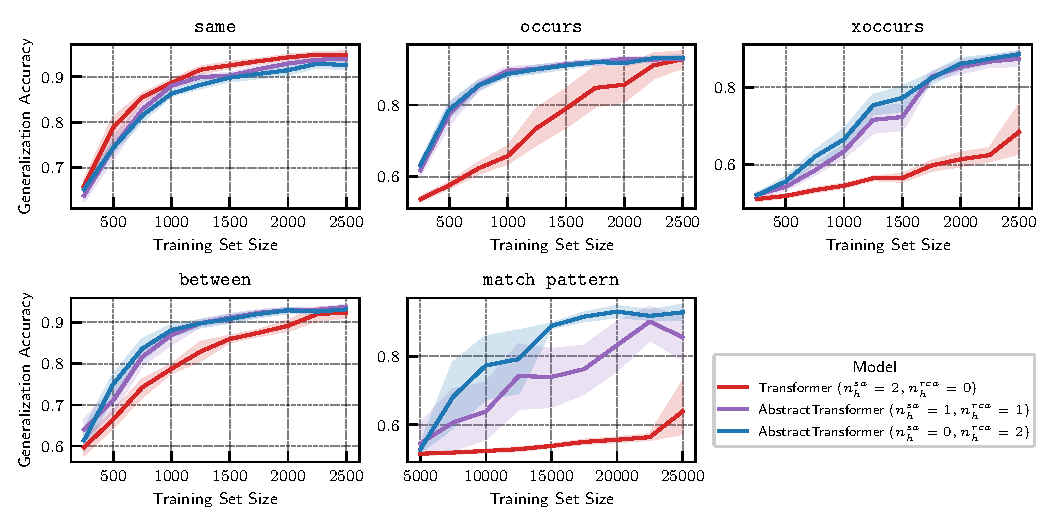
\includegraphics[width=\textwidth]{figs/experiments/relgames_learning_curves.pdf}
    \caption{}\label{fig:relgames_learning_curves}
\end{figure}

\subsection{Improved ``reasoning'' ability in sequence-to-sequence tasks: Mathematical Problem Solving}\label{ssec:math}

Show that we retain the benefits (even exceed?) of standard Abstractor on Seq2Seq tasks which the Abstractor also supports. Here, we can compare to the original Abstractor (i.e., it would be one of our baselines).

...

Motivate language modeling as the next set of experiments: this is something the original Abstractor could not be applied to directly, and the original paper did not tackle.

\begin{figure}
    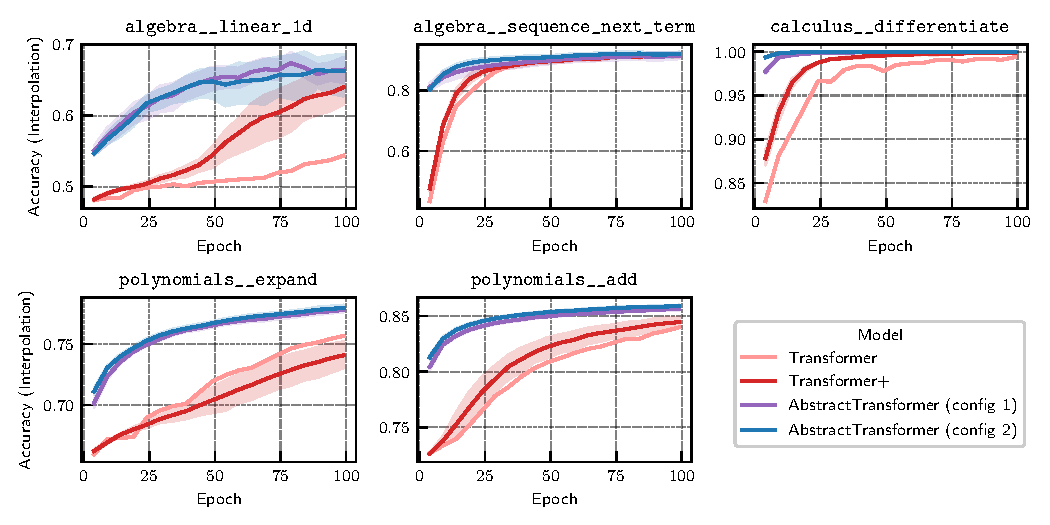
\includegraphics[width=\textwidth]{figs/experiments/math_training_curves_interpolation.pdf}
    \caption{}\label{fig:math_training_curves_interpolation}
\end{figure}

\subsection{Language Modeling: Tiny stories}\label{ssec:tiny_stories}

perhaps: [think about how to frame this section] 

- note that we are open-sourcing model weights
- modern LLM applications include varied and multi-modal tasks, so we conjecture that having more flexible [computational units] like RCA available to an LLM may lead to [performance improvements]. this is seen in the math and vision experiments, for e.g.
- so far, we haven't been able to spend too much time tinkering to find good hyperpams (which the problem is sensitive to). given more computational resources, this may be worthwhile...


\subsection{Multi-modality and potential in vision tasks: ImageNet}\label{ssec:imagenett}
\aanote{how is the acronym ``VAT''? Better than ViAT? VisAT? (Vision Transformer is ViT)}
